% /Users/philchodrow/.../main.tex
% RevTeX 4.2 minimal starter document

\documentclass[aps,pre,reprint,superscriptaddress,nofootinbib]{revtex4-2}
% \documentclass[aps,pre,reprint,superscriptaddress,nofootinbib,draft]{revtex4-2}


\usepackage{amsmath,amssymb,bm}
\usepackage{graphicx}
\usepackage{hyperref}
\usepackage{cleveref}
\hypersetup{colorlinks=true,linkcolor=blue,citecolor=blue,urlcolor=blue}


\newcommand{\paren}[1]{\left( #1 \right)}
\newcommand{\brackets}[1]{\left\langle #1 \right\rangle}
\newcommand{\squarebrackets}[1]{\left[ #1 \right]}
\newcommand{\prob}{\mathbb{P}}

\newcommand{\phil}[1]{\textcolor{blue}{PC: #1}}
\newcommand{\violet}[1]{\textcolor{red}{VR: #1}}
\newcommand{\frannie}[1]{\textcolor{green}{FC: #1}}

\begin{document}

\title{Growing Hypergraphs with Node Labels}
\author{Francis Cataldo$^*$}
\affiliation{Department of Computer Science, Middlebury College, Middlebury, VT, USA}
\author{Violet Ross$^*$}
\affiliation{Department of Computer Science, University of Colorado at Boulder, Boulder, CO, USA}
\author{Philip S. Chodrow}
\affiliation{Department of Computer Science, Middlebury College, Middlebury, VT, USA}


\date{\today}
\begin{abstract}
    We study a generative mechanistic model of hypergraph growth in which nodes possess binary labels which generalizes prior work on edge-copying growing hypergraphs.  
    Edges form in this model as noisy copies of previous edges, where the transmission of nodes from one edge to the next depends on the labels. 
    We derive a power law for the degree distribution in this model and describe the long-term dynamics of the joint distribution of labels contained in edges. 
    We then demonstrate that this model can be learned from data: we can both estimate the parameters of the model via (stochastic) expectation maximzation and perform community detection of the node labels via maximum-likelihood estimation. 
\end{abstract}

\maketitle

\def\thefootnote{*}\footnotetext{Equal author contributions}\def\thefootnote{\arabic{footnote}}


% \def\thefootnote{*}\footnotetext{These authors contributed equally to this work}\def\thefootnote{\arabic{footnote}}

\section{Introduction}

    Hypergraphs provide a natural, flexible data representation for complex systems with polyadic (multi-way) interactions, such as social interactions (both in-person \cite{mastrandrea2015contact} and online \cite{bensonSimplicialClosureHigherorder2018}), academic co-authorship \cite{wu2022hypergraph}, and ecological systems \cite{levine2017beyond}. 
    Much recent work has emphasized the importance of faithfully representing polyadic structure rather than reducing it to dyadic interactions \cite{battistonNetworksPairwiseInteractions2020,bick2023higher}, though recent work has shown that some purportedly higher-order dynamics can be faithfully represented on dyadic networks under appropriate models \cite{peixoto2026graphs}.

    % MORE HIGHER ORDER HERE
    Much attention in the theory of (hyper)graph mining has focused on developing novel techniques for community detection (also often called \emph{clustering} or \emph{partitioning}). 
    Many but not all of these methods can be viewed as exact or approximate inference algorithms for stochastic generative models. 
    A stochastic generative model is a parametrized probability distribution defined over hypergraphs. 
    In one standard framework, a set $\nodes$ of $n$ nodes is initialized along with a vector $\vz \in [k]^n$ that assigns to each node one of $k$ community labels. 
    One then forms the edge set $\edges$ iteratively by visiting each subset $R \subseteq \nodes$ and independently assigning $a_R$ (possibly repeated) edges to $R$ according to a distribution $p(a_R | \vz_R, \theta)$, where $\vz_R$ is the vector of labels of the nodes in $R$ and $\theta$ is a set of model parameters.
    This results in a probability distribution over hypergraphs which can be factorized into a product of edge probabilities conditioned on the node labels and model parameters: 
    \begin{align}
        p(\hypergraph | \vz, \theta) = \prod_{R \subseteq \nodes} p(a_R | \vz_R, \theta) \;. \label{eq:edge-independence}
    \end{align}
    Many generative models for community detection fall into this category, including hypergraph stochastic blockmodels \cite{chodrowGenerativeHypergraphClustering2021,ruggeriCommunityDetectionLarge2023,kim2018stochastic} and some generalizations \cite{badalyanStructureInferenceHypergraphs2024,hood2026broad}.
    The conditional independence property \cref{eq:edge-independence} is extremely useful for computation, as factorizability of the likelihood enables many efficiencies in various inference algorithms, including approximate maximum-likelihood estimation via direct optimization \cite{chodrowGenerativeHypergraphClustering2021} or expectation-maximization \cite{ruggeriCommunityDetectionLarge2023}; spectral methods \cite{chodrowNonbacktrackingSpectralClustering2023,fernandez2026achieving,li2026higher}; and message passing \cite{ruggeri2024message}. 
    Another recent optimization-based approach \cite{kritschgauCommunityDetectionHypergraphs2024} is equivalent to a microcanonical version of the stochastic blockmodel, which satisfies an asymptotic form of edge-independence in the large sparse limit.
    Even a recent latent-space model \cite{yuModelingHypergraphsDiversity2025} treats edges as independent samples, albeit from a very differently stochastic generating process. 
    
    Edge independence, however, is a strong and often unrealistic assumption for modeling hypergraph data. 
    A parallel line of work has found that polyadic data sets often contain significant edge correlations \cite{bensonSimplicialClosureHigherorder2018,landrySimplicialityHigherorderNetworks2024,leeHowHyperedgesOverlap2021}, typically in the form of \emph{similarity between interactions}.
    When an interaction occurs on a set $R \subseteq \nodes$, this increases the likelihood of observing a new interaction on a set $S \subseteq \nodes$ correlated with $R$ in the sense that $R\cap S$ is larger than would be expected by chance. 
    These overlaps can be shown to effect the kinds of dynamics which can unfold on the hypergraph \cite{maliziaHyperedgeOverlapDrives2025,lamata2025hyperedge}. 
    Several generative models for the growth of hypergraphs with edge-dependence have been proposed \cite{bensonSequencesSets2018,avinRandomPreferentialAttachment2019,heEdgeCorrelationsLink2025,leeTHyMeTemporalHypergraph2021,leeTemporalHypergraphMotifs2023}. 
    Several of these models express dependence through a copying or recombination mechanism, in which nodes collected from one or more existing hyperedges are gathered and noisily copied into a new edge as a block.  

    % Phil prewriting got down to here.

    In this paper, we introduce a model of binary node-labeled hypergraphs in which edges form via a noisy copying interaction which depends the labels. 
    Our work is organized as follows. 
    In \Cref{sec:model-description}, we describe our model and derive limiting descriptions of the joint distribution of node labels within a given edge, as well as the degree distribution of the hypergraph.
    Evaluating the likelihood of our model requires marginalizing over a set of latent variables governing the noisy copy mechanism, which is computationally expensive. 
    To estimate our model's parameters when node labels are known, we therefore describe a stochastic expectation-maximization algorithm in which each iteration has sublinear cost in the number of edges for sparse hypergraphs.
    We also describe a community detection algorithm for estimating node labels via simulated annealing. 
    In \Cref{sec:results} we demonstrate our algorithms on synthetic and empirical data. 
    We show that, on synthetic data sampled from our model, our stochastic expectation maximization algorithm is both consistent and scalable, and that our simulated annealing algorithm for community detection, though computationally expensive, outperforms other standard methods. 
    On empirical data, our parameter estimatates yield insight into the mechanisms governing edge formation
    Our community detection achieves competitive recovery of observed metadata labels on some data sets known to be challenging to other community detection methods.
    We conclude with some discussion of future directions for models of node-labeled hypergraphs with edge-dependence. 

\section{Model Description} \label{sec:model-description}

    \begin{figure}
        \centering 
        \caption{PLACEHOLDER: schematic of the model here, or alternatively a sample from the model.}
    \end{figure}

    \begin{figure}
        \centering 
        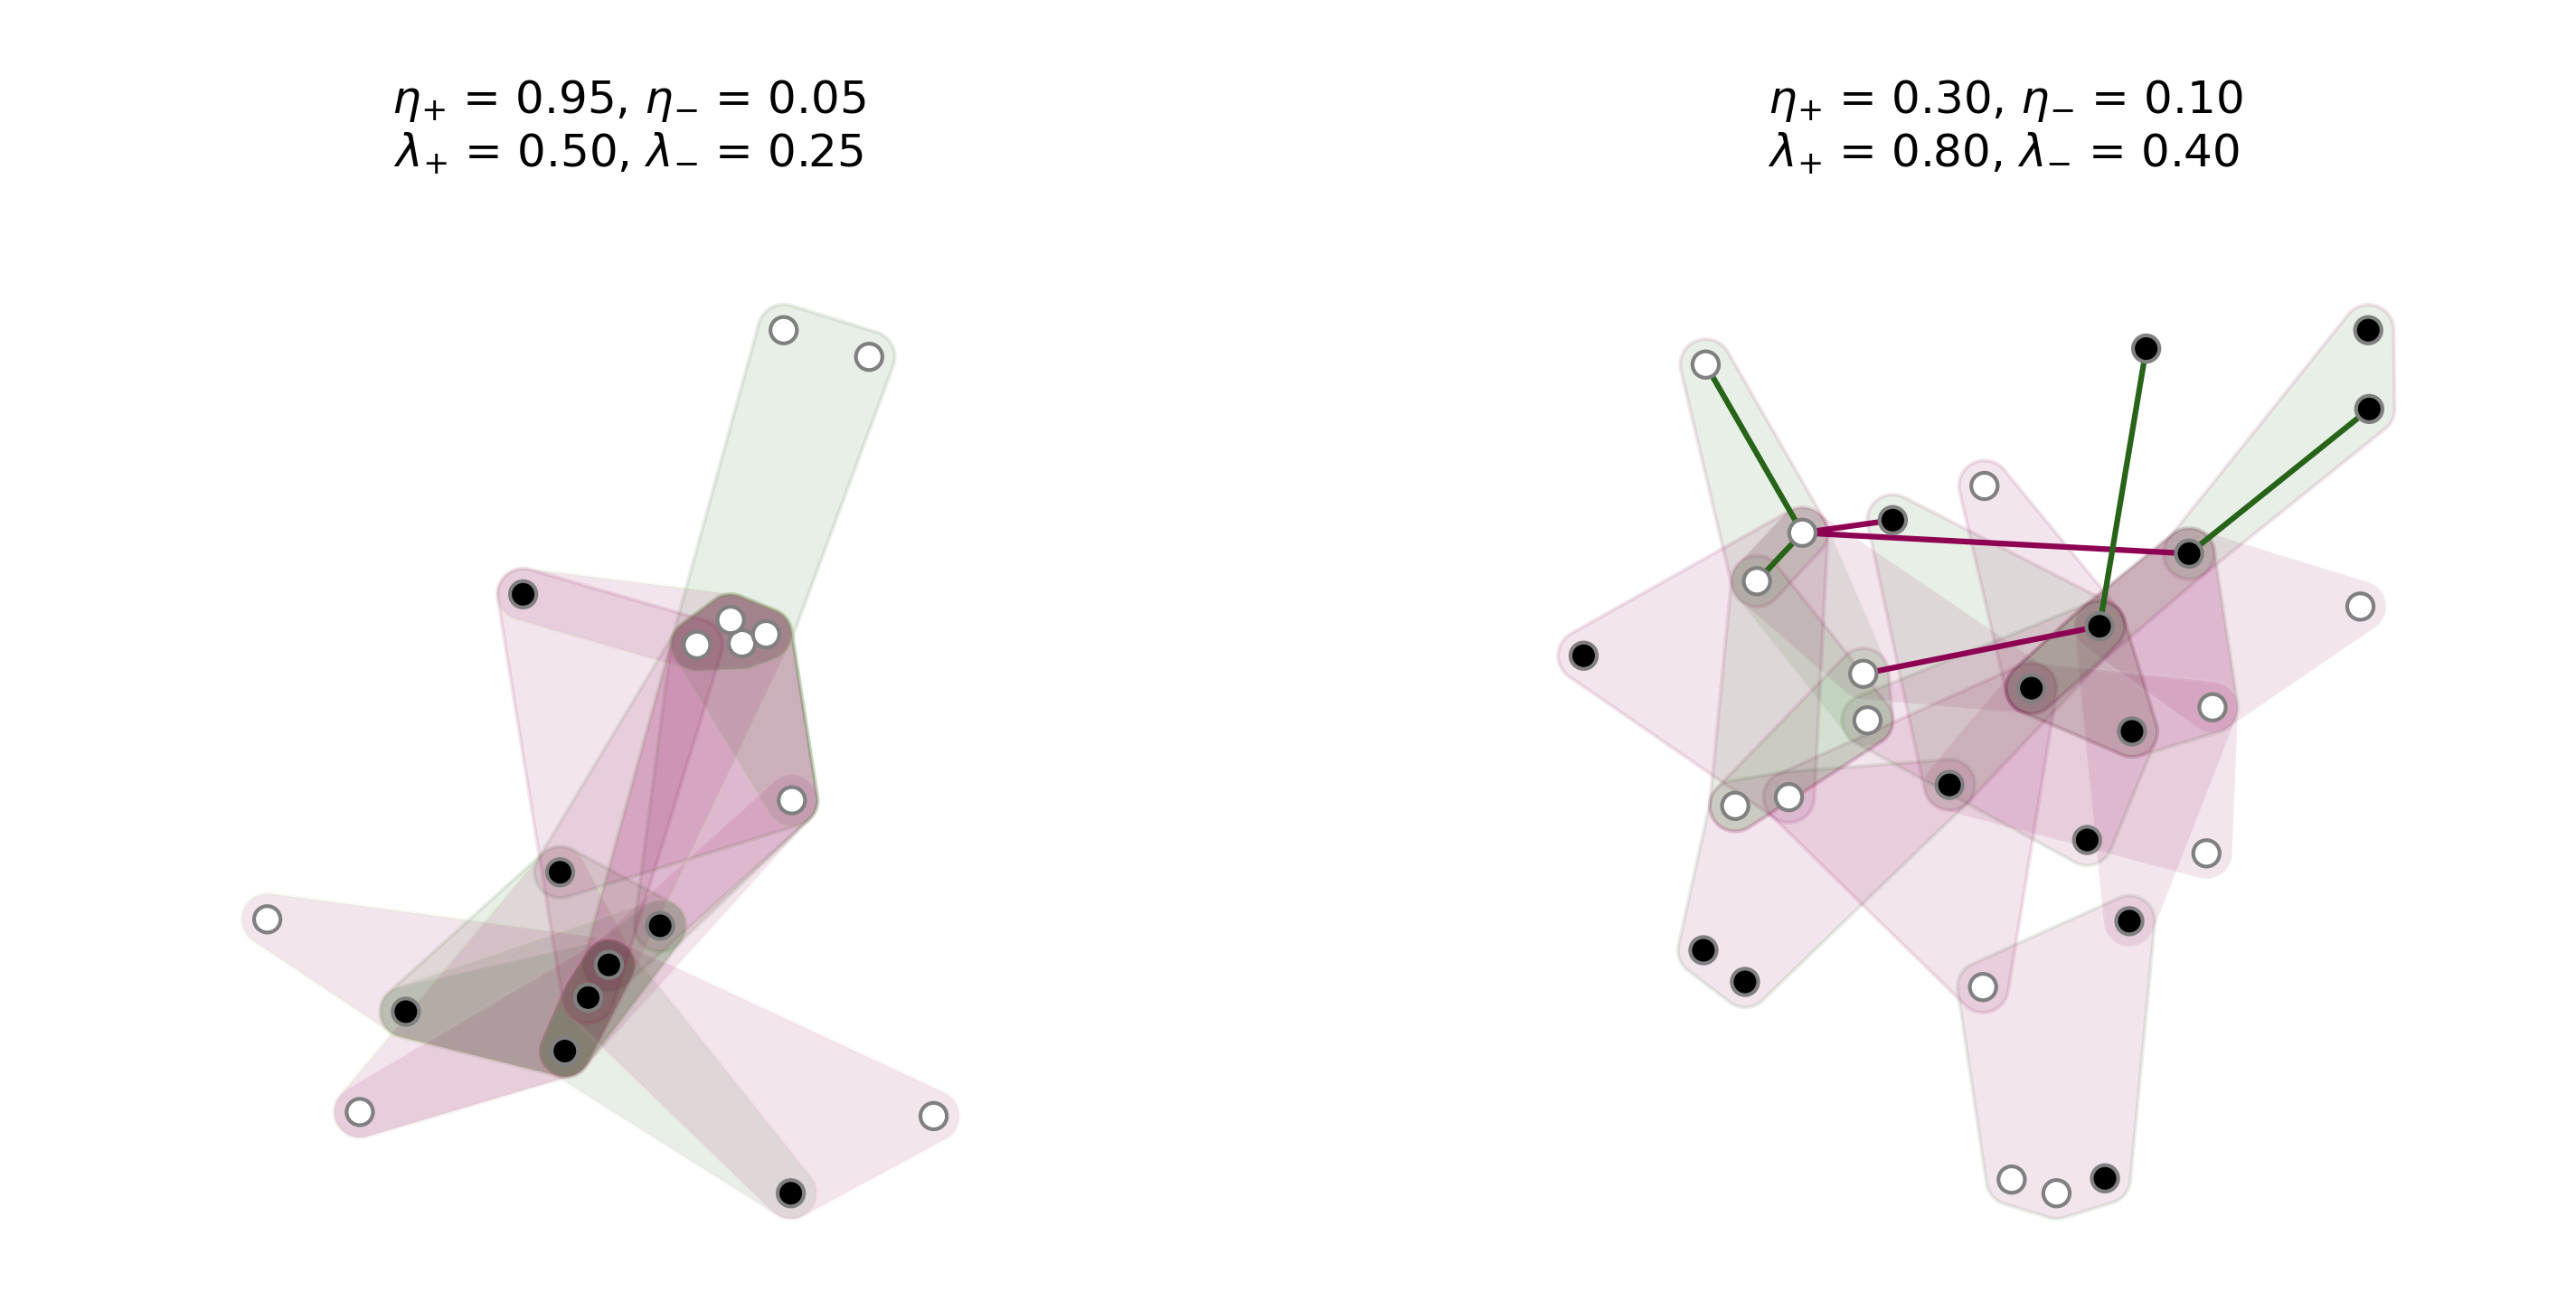
\includegraphics[width=0.48\textwidth]{../fig/hypergraph_viz.png}
        \caption{Two samples from our model. 
        Node color corresponds to community label.
        Label-homogeneous edges are shown in green, while label-heterogeneous edges are shown in pink.
        In each case, $\samelabelnovelrate{} = 0.5$, $\opplabelnovelrate{} = 0.25$, and the remaining parameters are as given. 
        The model begins with two disjoint label-homogeneous edges and is run for 25 timesteps.
        } \label{fig:examples}
    \end{figure}

    Our model builds on the Hyperedge Copy Model (HCM) of He et al. \cite{heEdgeCorrelationsLink2025}. 
    In their model, edges form through a combination of three distinct steps: a copy step, in which a previous edge is sampled and imperfectly copied; an extant node addition step, in which new nodes are added to the new edge from the existing node set; and a new node addition step, in which new nodes are added to the new edge from outside the existing node set.
    Our model replicates these mechanisms but adds label-aware parameters to regulate each. 

    Formally, a state of our model at time $t$ is a hypergraph $\at{\hypergraph}{t} = \paren{\at{\nodes}{t}, \at{\edges}{t}}$, where $\nodes$ is the set of nodes and $\edges$ is the set of hyperedges. 
    Each node $\node \in \nodes$ has a binary label $z_{\node} \in \{0, 1\}$.
    We let $\bar{z} = 1 - z$ denote the opposite label of $z$.
    At timestep $t$, add edge $\newedge$ to $\at{\edges}{t}$ to obtain $\at{\edges}{t+1}$, where $\newedge$ is formed according to the following three-step process:
    \begin{itemize}
        \item 
            \textbf{Edge-Copying}: An edge $\seededge$ is sampled uniformly at random from $\at{\edges}{t - 1}$, and a node $\focalnode$ is sampled uniformly at random from $\seededge$. 
            Then, each node $\node$ in $\seededge$ is included in $\newedge$ with probability $\samelabelcopyrate{}$ if $z_{\node} = z_{\focalnode}$ and with probability $\opplabelcopyrate{}$ if $z_{\node} \neq z_{\focalnode}$.
        \item 
            \textbf{Extant Node Addition}: We sample $\extantnodesinedge_{z_\focalnode}$ nodes from $\nodes \setminus \seededge$ with label $z_\focalnode$ and add them to $\newedge$, where $\extantnodesinedge_z$ is a Poisson random variable with mean $\samelabelextantrate{}$. 
            We similarly sample $\extantnodesinedge_{\bar{z}_\focalnode}$ nodes from $\nodes \setminus \seededge$ with label $\bar{z}_\focalnode$ and add them to $\newedge$, where $\extantnodesinedge_{\bar{z}_\focalnode}$ is a Poisson random variable with mean $\opplabelextantrate{}$.
        \item \textbf{Novel Node Addition}: We sample $\novelnodesinedge_{z_\focalnode}$ new nodes with label $z_\focalnode$ and add them to $\newedge$, where $\novelnodesinedge_z$ is a Poisson random variable with mean $\samelabelnovelrate{}$.
            We similarly sample $\novelnodesinedge_{\bar{z}_\focalnode}$ new nodes with label $\bar{z}_\focalnode$ and add them to $\newedge$, where $\novelnodesinedge_{\bar{z}_\focalnode}$ is a Poisson random variable with mean $\opplabelnovelrate{}$.   
    \end{itemize}
    In our simulations we initialize $\at{\hypergraph}{0}$ with a single edge containing one node of each label, but any combination of hypergraph and node labels can be used as an initial condition. 
    Both our simulations and our statistical inference techniques (described below) were carried using the XGI package for polyadic data analysis in Python \cite{landryXGIPythonPackage2023}. 



\subsection{Asymptotic Properties} \label{sec:asymptotics}

    \subsubsection{Joint Distribution of Labels in Edges} \label{sec:joint-distribution}

    \begin{figure*}[t]
        \centering
        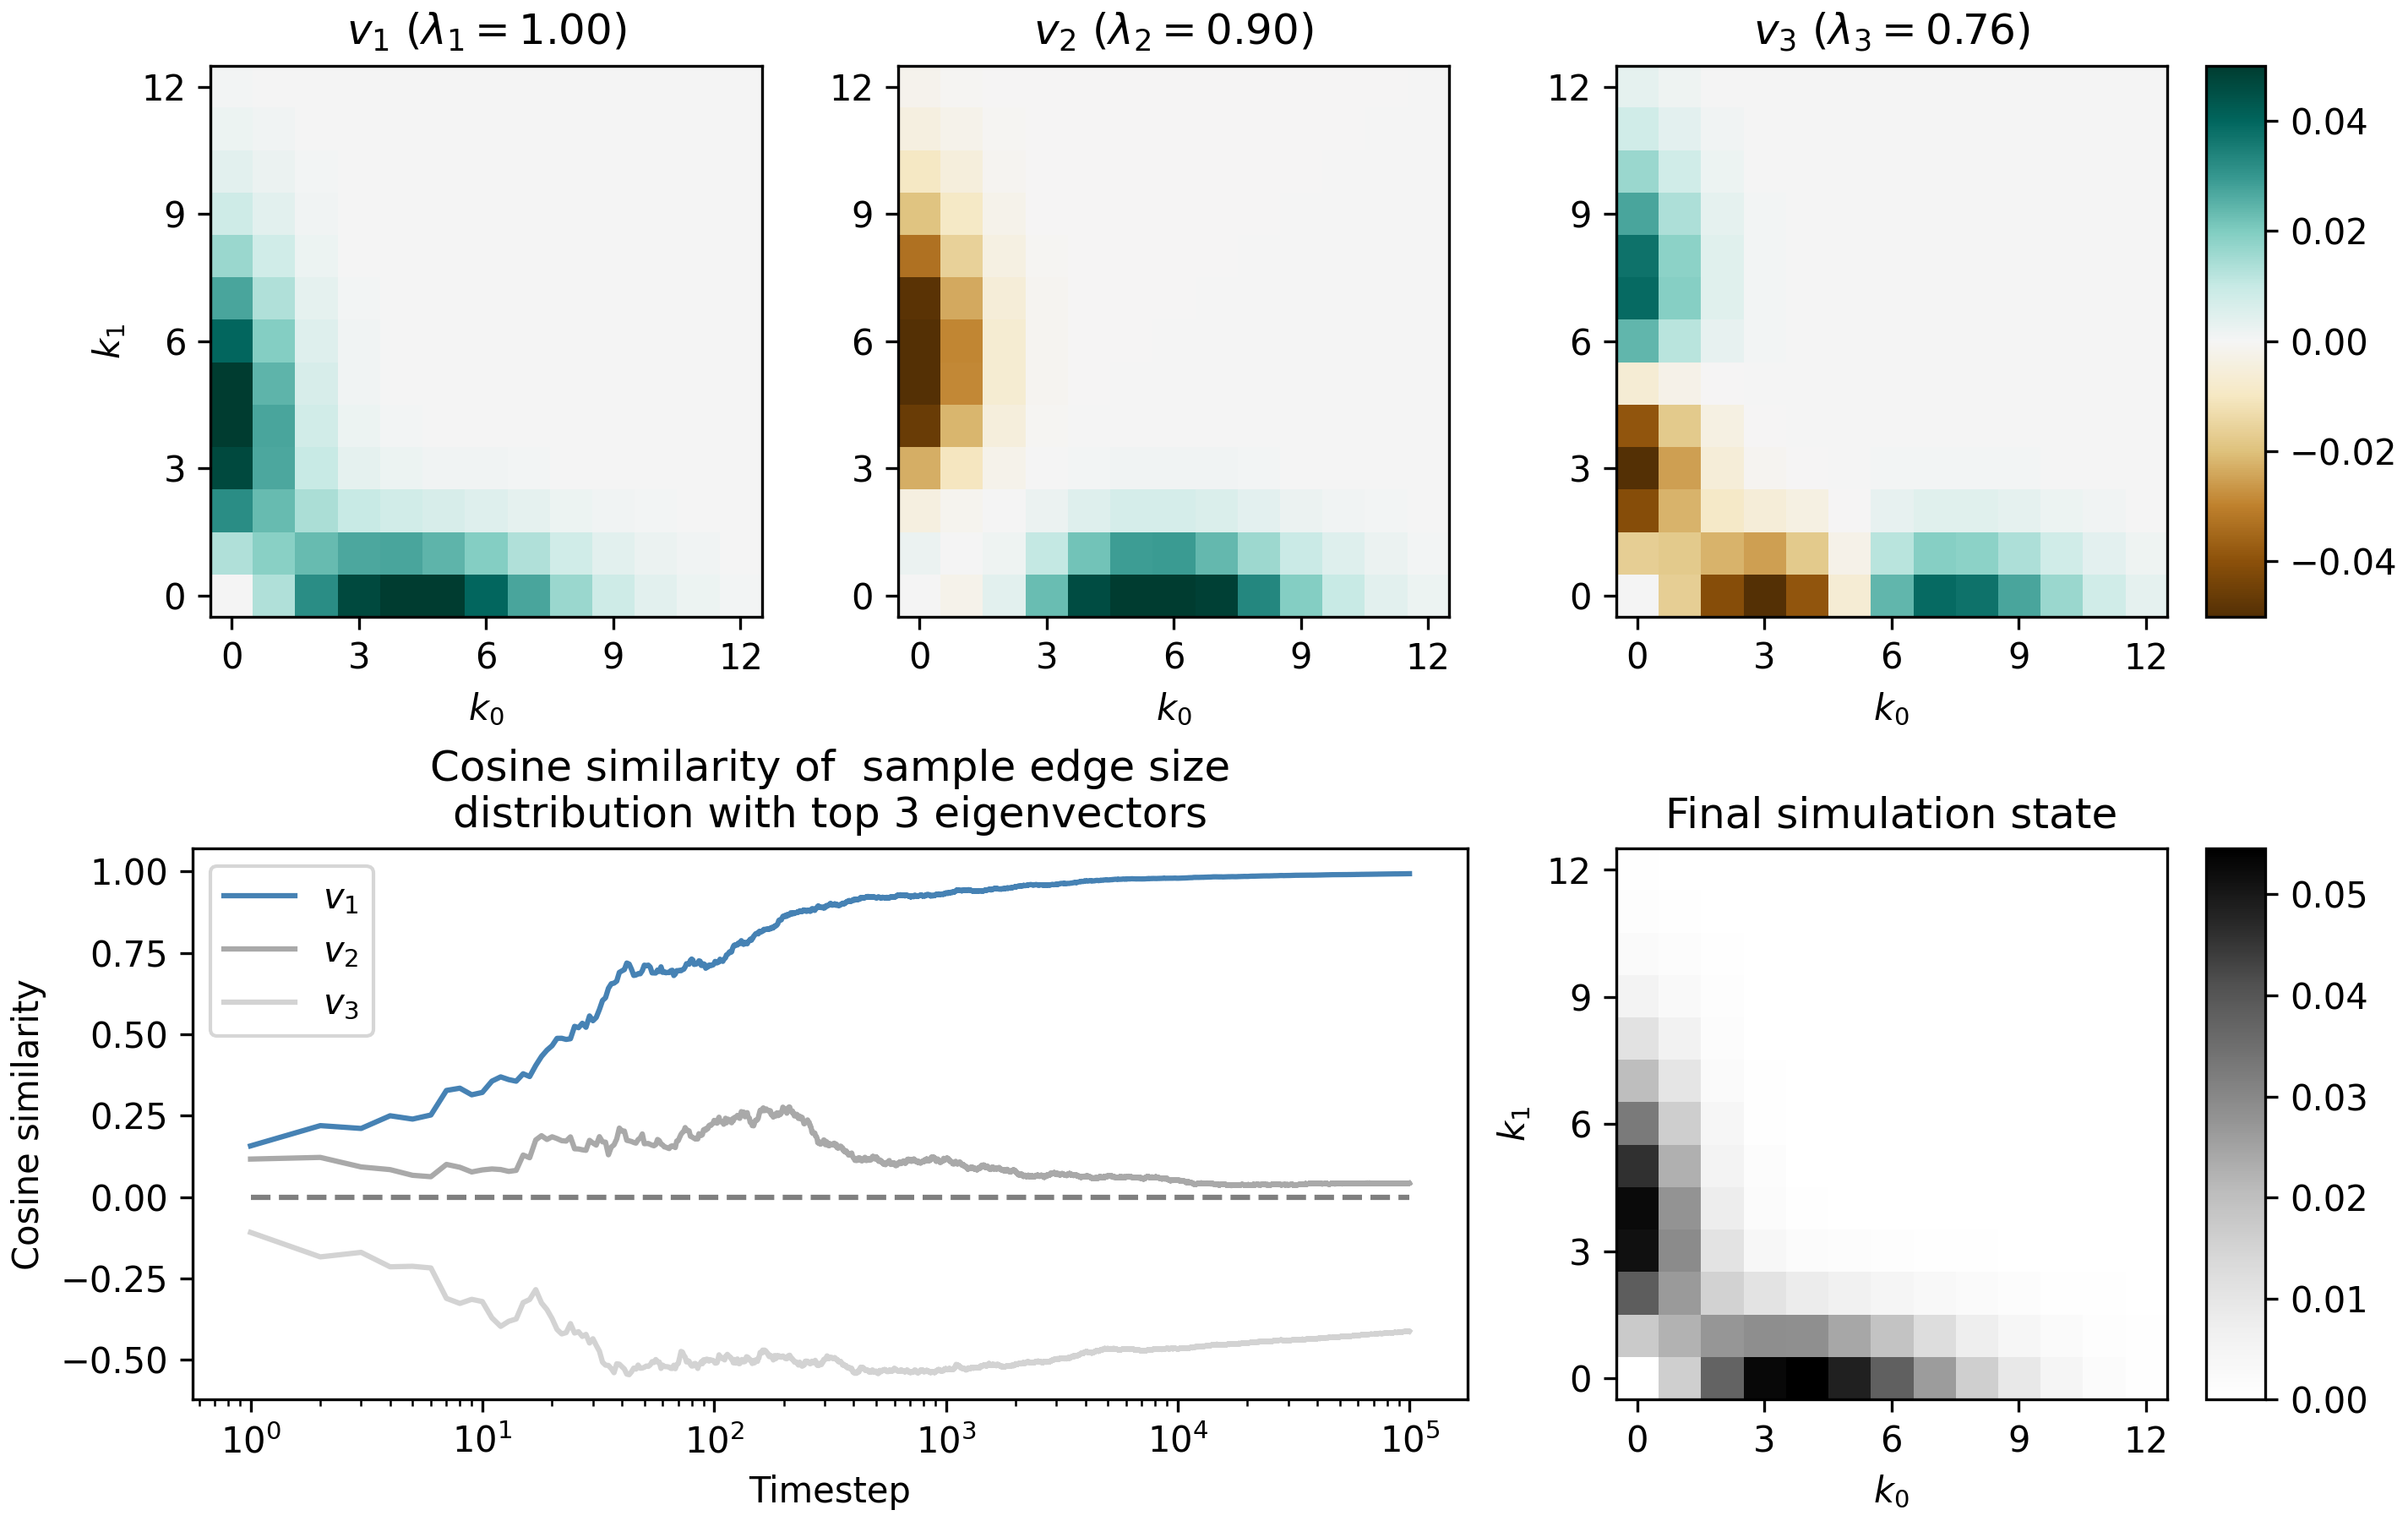
\includegraphics[width=1\textwidth]{../fig/linear_map_eigenvectors.png}
        \caption{
            Visualization of the long-run dynamics of our model, for parameters. 
            (a): Spectral gap $1 - \lambda_2$ of the linear map $T$ as a function of $\samelabelcopyrate{}$ and $\opplabelcopyrate{}$ for fixed parameter values $\samelabelextantrate{} = 0.5$, $\opplabelextantrate{} = \opplabelnovelrate{}3$, $\samelabelnovelrate{} = 0.4$ and $\opplabelnovelrate{} = 0.2$. 
            The highlighted values $\samelabelcopyrate{} = 0.8$ and $\opplabelcopyrate{} = 0.1$ are used in the remainder of the visualization. 
            (b): Leading eigenvector $\mathbf{v}_1$ of $T$, describing the stationary joint distribution $\at{\jointdist}{\infty} \paren{k_0, k_1}$ of label counts in edges.
            (c): Second eigenvector $\mathbf{v}_2$ of $T$. 
            The transients of the model dynamics are dominated by the subspace spanned by $\mathbf{v}_1$ and $\mathbf{v}_2$. 
            (d): Euclidean projections of the simulated joint distribution $\at{\jointdist}{t} \paren{k_0, k_1}$ onto the eigenvectors $\mathbf{v}_1$ and $\mathbf{v}_2$ during a simulation run with $10^7$ timesteps. 
            At each time point, we aggregate the most recent $1,000$ edges to compute the joint distribution in order to approximate an ``instantaneous'' simulation state. 
            (e): Empirical joint distribution $\at{\jointdist}{t} \paren{k_0, k_1}$ aggregated across $10^7$ timesteps. 
        }
        \label{fig:dynamics-eigenvectors}
    \end{figure*}

    The asymptotics of this model can be described in terms of the joint distribution $p_{K_0, K_1}(k_0, k_1)$ of nodes of labels 0 and 1 in a uniformly random edge. 
    This joint distribution can be obtained as the leading eigenvector of a linear map. 
    Let $p^{(t)}(k_0, k_1)$ be the joint distribution of label counts in a uniformly random edge after $t$ timesteps. 
    Then, the probability $q(k_0', k_1')$ of realizing an edge with $k_0'$ nodes of label 0 and $k_1'$ nodes of label 1 at time $t+1$ is given by 
    \begin{align*}
        q(k_0', k_1') = \sum_{k_0, k_1} T(k_0', k_1' | k_0, k_1)p^{(t)}(k_0, k_1)  \;,
    \end{align*}
    where $T(k_0', k_1' | k_0, k_1)$ gives the probability that the edge $e$ realized in step $t+1$ has $k_0'$ nodes of label 0 and $k_1'$ nodes of label 1 given that the edge $f$ sampled to form $e$ has $k_0$ nodes of label 0 and $k_1$ nodes of label 1.
    At stationarity, we must have $q(k_0', k_1') = p^{(t)}(k_0', k_1') = p^{(t+1)}(k_0', k_1')$, so the stationarity condition can be obtained by solving the linear system 
    \begin{align*}
        \at{\jointdist}{t+1} \paren{k_0', k_1'} = \sum_{k_0, k_1} T(k_0', k_1' | k_0, k_1)\at{\jointdist}{t} \paren{k_0, k_1}  \;.
    \end{align*}
    The stationary joint distribution $\at{\jointdist}{\infty} \paren{k_0, k_1}$ is therefore given by the leading eigenvector of the doubly-indexed matrix $T$ with entries $T(k_0', k_1' | k_0, k_1)$.
    The entries of this matrix can be computed analytically. 
    Conditional on choosing an edge $f$ with $k_0$ nodes of label 0 and $k_1$ nodes of label 1, a node of label $z$ is selected as the seed node $u$ with probability $\frac{k_z}{k_0 + k_1}$.
    Then, the number of nodes of labels $z$ and $\bar{z}$ in $e$ have distributions
    \begin{align*}
        k_z' &\sim 1 + \text{Binom}\paren{k_z - 1, \samelabelcopyrate{}} + \text{Poisson}(\samelabelextantrate{} + \samelabelnovelrate{}) \;, \\
        k_{\bar{z}}' &\sim \text{Binom}\paren{k_{\bar{z}}, \opplabelcopyrate{}} + \text{Poisson}(\opplabelextantrate{} + \opplabelnovelrate{}) \;.
    \end{align*}
    The probability of obtaining $k_0'$ nodes of label 0, conditioning on $k_0$ and $k_1$, is 
    \begin{widetext}
        \begin{align*}
            t(k_0' | k_0, k_1) =& \frac{k_0}{k_0 + k_1} \sum_{i=0}^{k_0' - 1} \binom{k_0 - 1}{i} \samelabelcopyrate{}^i (1 - \samelabelcopyrate{})^{k_0 - 1 - i} 
            e^{-(\samelabelextantrate{} + \samelabelnovelrate{})} \frac{(\samelabelextantrate{} + \samelabelnovelrate{})^{k_0' - 1 - i}}{(k_0' - 1 - i)!}  + \\ 
            & \frac{k_1}{k_0 + k_1} \sum_{i=0}^{k_0'} \binom{k_0}{i} \opplabelcopyrate{}^i (1 - \opplabelcopyrate{})^{k_0 - i} 
            e^{-(\opplabelextantrate{} + \opplabelnovelrate{})} \frac{(\opplabelextantrate{} + \opplabelnovelrate{})^{k_0' - i}}{(k_0' - i)!}\;.
        \end{align*}
    \end{widetext}
    A parallel expression describes $t(k_1' | k_0, k_1)$, and the transition matrix entries are given by the product 
    \begin{align*}
        T(k_0', k_1' | k_0, k_1) = t(k_0' | k_0, k_1) t(k_1' | k_0, k_1) \;.
    \end{align*}
    In \Cref{fig:dynamics-eigenvectors}, we show projections of the joint distribution $\at{\jointdist}{t} \paren{k_0, k_1}$ onto the top two eigenvectors of the matrix $T$ during a simulation run. 
    These eigenvectors are computed numerically. 
    The Perron eigenvector $v_1$ with eigenvalue $1$ corresponds to the stationary distribution $\at{\jointdist}{\infty} \paren{k_0, k_1}$. 
    The second eigenvector $v_2$ with eigenvalue $\lambda_2 < 1$ corresponds to the slowest-decaying transient in the dynamics of $\at{\jointdist}{t} \paren{k_0, k_1}$.
    The spectral gap $1 - \lambda_2$ is relatively small, indicating slow transients in the subspace spanned by $v_1$ and $v_2$.

\subsubsection{Degree Distribution} \label{sec:degree-distribution}

    \begin{figure}[t]
        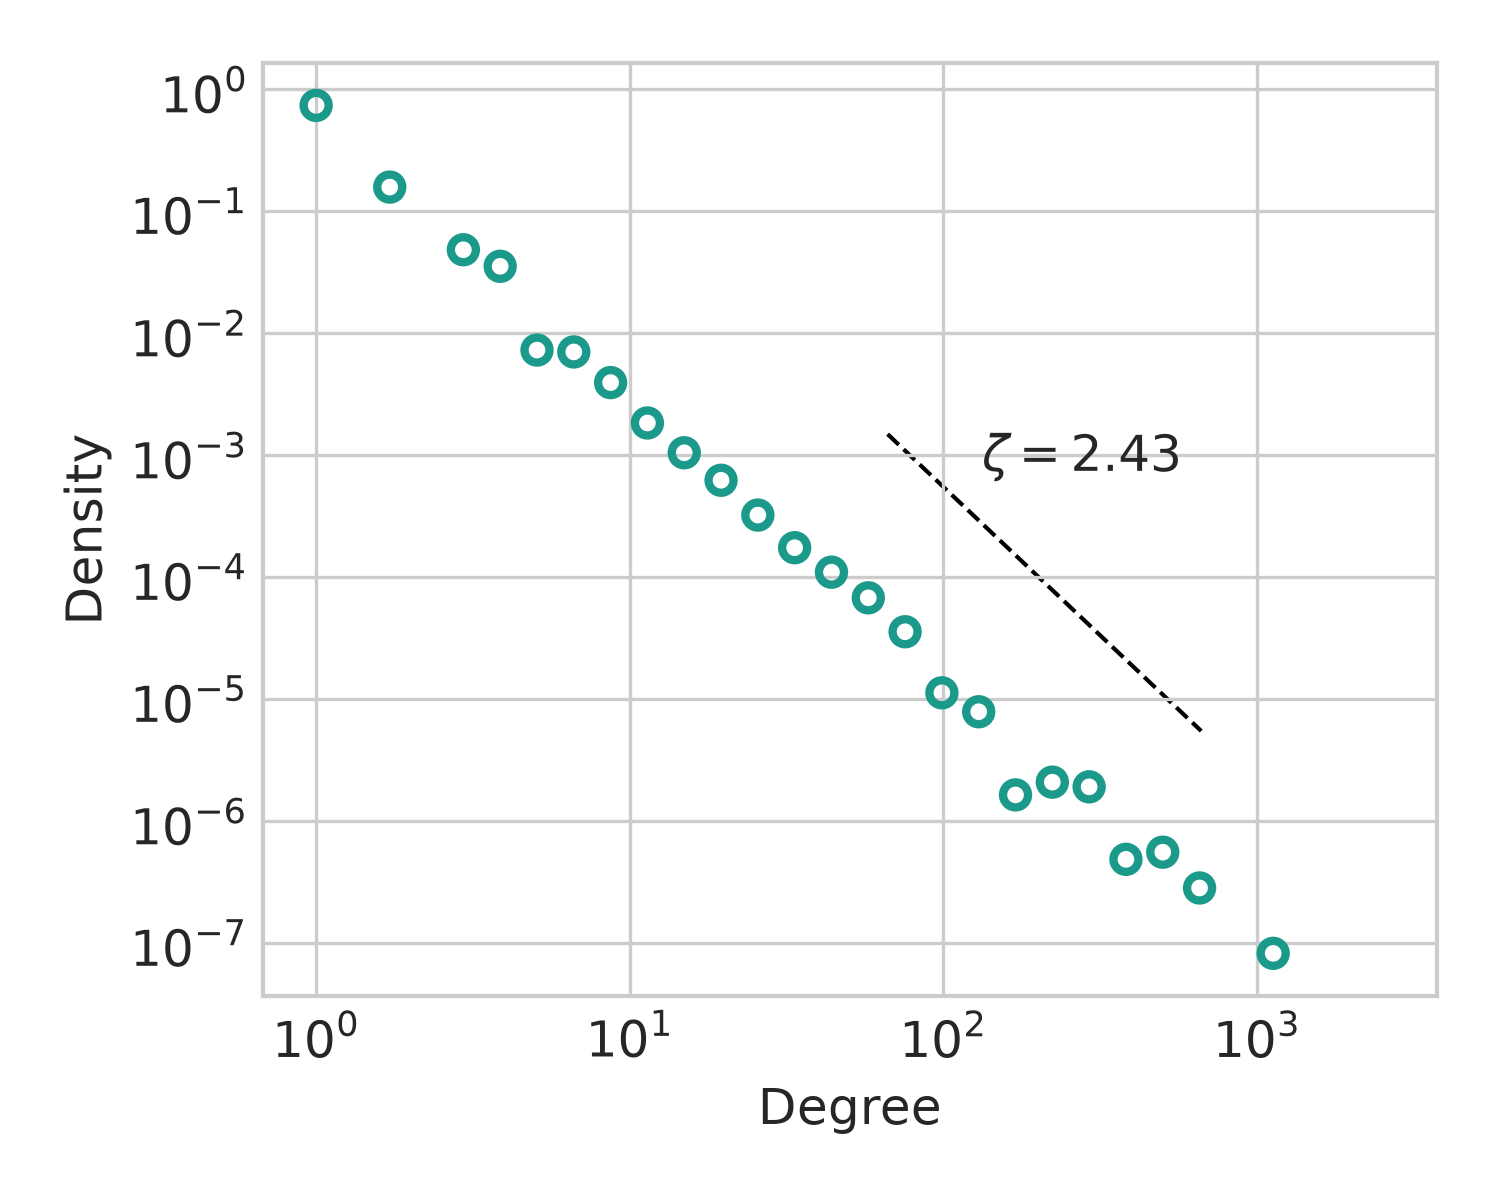
\includegraphics[width=0.5\textwidth]{../fig/degree_distribution.png}
        \caption{
            Degree distribution from model simulation of $10^4$ edges (points) and theoretical power law (line) with exponent given by \Cref{eq:power-law-exponent}. 
            The parameters in this experiment are $\samelabelcopyrate{} = 0.7, \opplabelcopyrate{} = 0.3, \samelabelextantrate{} = 0.5, \opplabelextantrate{} = \opplabelnovelrate{}3, \samelabelnovelrate{} = 0.2, \opplabelnovelrate{} = 0.1$.
            }
        \label{fig:degrees}
    \end{figure}

    The degree distribution of a hypergraph generated from our model follows an asymptotic power law with an exponent which can be computed in closed form from the model parameters and the stationary joint distribution $\at{\jointdist}{\infty} \paren{k_0, k_1}$. 
    Our derivation follows that of He et al. \cite{heEdgeCorrelationsLink2025}, which in turn is based on a derivation by Mitzenmacher \cite{mitzenmacherBriefHistoryGenerative2004}. 
    To carry out the argument, we require a mean-field assumption that, when a node $v$ is selected from edge $f$ in the edge-sampling step, the degree $d$ of $v$ is independent of the ratio $\frac{k_0}{k}$ of label-0 nodes in the edge $\seededge$ sampled to form the new edge $\newedge$.
    
    Under this assumption, it is possible to show that the degree distribution follows a power law with exponent
    \begin{align}
        \zeta &= 1 + \frac{\brackets{k}}{1 + \samelabelcopyrate{}(\rho_{00} + \rho_{11} - 1) + 2\opplabelcopyrate{} \rho_{01}} \label{eq:power-law-exponent}\\ 
        \rho_{ij} &= \brackets{\frac{k_i k_j}{k}} \;. \nonumber
    \end{align}
    In the expression for $\rho_{ij}$ (and for $\brackets{k}$) the expectation is taken with respect to the stationary joint distribution $\at{\jointdist}{\infty} \paren{k_0, k_1}$.
    Here, $\totalnovelrate{}$ can be interpreted as the expected number of novel nodes added per new edge, while $\sigma$ can be interpreted as the expected number of nodes copied into a new edge from the sampled edge, normalized by the average degree of a node in the hypergraph.
    

    \subsubsection{Community Structure}

        \emph{Show a plot describing how the modularity of the clique projection varies by parameter, and perhaps some sample hypergraphs with associated partitions. }

        

\section{Model Inference}

\phil{Phil needs to establish standardized notation in this section.}

\subsection{Parameter Estimation via Stochastic EM}

\phil{Violet, this is your spot! Descriptions of methods/algorithms should go here, results are for later. }

    We first consider the problem of learning the parameter vector $\paramvector = (\samelabelcopyrate{}, \opplabelcopyrate{}, \samelabelextantrate{}, \opplabelextantrate{}, \opplabelnovelrate{}, \opplabelnovelrate{})$ given an observed hypergraph $\hypergraph$ with sequential edge indices and known node labels $\vz$.
    We aim to do this via maximum-likelihood estimation. 
    Computing the complete data likelihood requires marginalizing over the model latent variables, which in this case are the edge $f$ and node $u$ selected at each timestep of the growth model to form the new edge $e$: 
    \begin{align}
        \prob(\hypergraph, \vz | \paramvector) = \prod_{t=1}^T \sum_{f \in \edges_{t - 1}} \sum_{u \in f} p(e | f, u, \vz, \paramvector) p(f,u| \edges_{t - 1}, \vz, \paramvector) \;. \label{eq:likelihood}
    \end{align}
    For notational simplicity, we have repressed the additional entries of $\vz$ introduced by the novel node addition step. 
    The requirement to sum over the latent variables at each timestep implies a computational cost to evaluate $\prob(\hypergraph, \vz | \paramvector)$ (or its derivatives) which is quadratic in the number of edges, making direct optimization of the likelihood expensive for data sets of even modest size. 
    Batch expectation-maximization \cite{dempster1977maximum}  is an alternative approach which maximizes the likelihood without explicitly computing \cref{eq:likelihood}, but even this approach requires forming a belief distribution over the values of all latent variables at each timestep, which again incurs quadratic cost. 
    
    We therefore use a stochastic expectation-maximization (SEM) algorithm \cite{cappeOnLineExpectationMaximization2009} to estimate the parameters $\paramvector$.
    Each iteration of the SEM algorithm consists of two steps: the E-step, in which exponentially-weighted moving averages of
    the sufficient statistics are calculated using the current parameter estimates, and the M-step, in which the parameter estimates are updated using the expected sufficient statistics. 

Suppose we have an observed variable $x$ and a hidden variable $h$. Let $f(x_i, h_i)$ be a function which computes a sufficient statistic for each of the parameters in $\theta$ and let $F_i(\hat{\theta}) = \mathbb{E}[f(x_i, h_i) | x_i]$ be the function which computes the expected sufficient statistic values given an observed $x_i$. Let $g$ be a function which computes the maximum likelihood estimate of $\theta$ from the sufficient statistics. Fix a sequence of learning rates $\ell^{(1)}, \ldots, \ell^{(t)}$. Each iteration, $t$, of SEM proceeds as follows.
    
\textbf{E step:} Sample an observation $x_i$ from the data uniformly at random. Compute the expected sufficient statistics $F_i(\hat{\theta}^{(t - 1)})$ using the randomly selected data point $x_i$ and the parameter estimates $\hat{\theta}^{(t - 1)}$ from the previous timestep. Generate an new estimate of sufficient statistics $s^{(t)}$ according to the update rule: $s^{(t)} = (1 - \ell^{(t)}) s^{(t - 1)} + \ell^{(t)}F_i(\hat{\theta}^{(t - 1)})$.
    
\textbf{M step:} Compute the new parameter estimates $\hat{\theta}^{(t)}$ from the updated sufficient statistics:
$\hat{\theta}^{(t)} = g(s^{(t)})$.
    
\subsubsection{Description of SEM on hypergraphs}
We use an SEM algorithm to estimate the parameters $\theta = (p, q, \totalnovelrate{}_{e, z_u}, \totalnovelrate{}_{e, \bar{z_u}}, \totalnovelrate{}_{e, z_n}, \totalnovelrate{}_{e, \bar{z_n}})$ used to generate a hypergraph $\mathcal{H}$ via the [MODEL NAME] model. At each timestep, we have an observed variable $e'$ (a hyperedge) and two hidden variables $u$ and $e$ (the node and the hyperedge that generated $e'$). Let $f$ be a function which computes a sufficient statistic for each of the parameters in $\theta$. Specifically, let
\begin{equation*}
    f(e, u, e') = (t_{z_u}, w_{z_u}, t_{\bar{z}_u}, w_{\bar{z}_u}, n_{e, z_u}, n_{e, \bar{z}_u}, n_{n, z_u}, n_{n, \bar{z}_u})
\end{equation*}
where $w_{z_u}$ is the number of nodes with label  $z_u$ in $e$, $w_{\bar{z}_u}$ is the number of nodes with the label $\bar{z}_r$ in $e$, $t_{z_u}$ and $t_{\bar{z}_u}$ are the numbers of nodes with label $z_u$ and $\bar{z}_r$, respectively, copied from $e$ to $e'$, $n_{e, z_u}$ and ${n_{e, \bar{z}_u}}$ are the numbers of external nodes with labels $z_u$ and $\bar{z}_r$ in $e'$, and $n_{n, z_u}$ and ${n_{n, \bar{z}_u}}$ are the numbers of new nodes with labels $z_u$ and $\bar{z}_r$ in $e'$. 
% The sufficiency of these statistics follows from standard results \cite{rice2007mathematical}. 
Then the function 
\begin{equation*}
    \begin{split}
        F_{e'}(\hat{\theta}^{(t - 1)}) &= \mathbb{E}[f(e, u, e') | e', \hat{\theta}^{(t - 1)}] \\
        &= \frac{\sum_{e \in \mathcal{E}_{\text{prev}}} \sum_{u \in e \cap e'} p(e, u, e' | \hat{\theta}^{(t - 1)}) f(e, u, e')}{\sum_{e \in \mathcal{E}_{\text{prev}}} \sum_{u \in e \cap e'} p(e, u, e' | \hat{\theta}^{(t - 1)}) } 
    \end{split}
\end{equation*}
computes the expected values of the sufficient statistics at time $t$ given edge $e'$. Finally, the maximum likelihood estimate of $\theta$ is given by
\begin{equation*}
    g(s^{(t)}) = \left( \frac{t_u}{w_{z_u}}, \frac{t_{\bar{z}_u}}{w_{\bar{z}_u}}, n_{e, z_u}, n_{e, \bar{z}_u}, n_{n, z_u}, n_{n, \bar{z}_u} \right).
\end{equation*}
Each iteration of our SEM algorithm for hypergraphs then proceeds following the E- and M-steps detailed above.



\subsection{Community Detection via MLE}

\phil{Frannie, this is your spot! Descriptions of methods/algorithms should go here, results are for later.}

We also used gradient descent with a continuous relaxation of the parameter labels \cite{pytorch}. 

We also did simulated annealing! \cite{kirkpatrickOptimizationSimulatedAnnealing1983}. 


\section{Results} \label{sec:results}

How did we do on real and synthetic data? 




\section{Conclusion}

    Future directions: 

    Edge relevance-decay. Background interaction events. Work on scalability of community detection and parameter estimation. 
    Models with multiple edge labels, e.g. planted partition (symmetric) models. 

\begin{acknowledgments}
    PSC acknowledges support from the National Science Foundation under DMS-2407058.
\end{acknowledgments}



\bibliographystyle{apsrev4-2}
\bibliography{refs} 

\appendix

\section{Appendix}

    

    \subsection{Power-Law Degree Distribution}


    Our derivation follows that of He et al. \cite{heEdgeCorrelationsLink2025}, which in turn is based on a derivation by Mitzenmacher \cite{mitzenmacherBriefHistoryGenerative2004}.

    At stationarity, the mean degree $\brackets{d}$ of a node satisfies 
    \begin{align}
        \brackets{d} = \frac{m}{n}\brackets{k} \;,
    \end{align}
    where $\brackets{k}$ is the mean edge size (computable from the stationary distribution $\jointdist \paren{k_1,k_2}$), $m$ is the number of edges, and $n$ is the number of nodes.
    In expectation, there are $\totalnovelrate{} \triangleq \opplabelnovelrate{} + \samelabelnovelrate{}$ new nodes added per new edge, which means that $\frac{m}{n} \to \frac{1}{\totalnovelrate{}}$ as $m, n \to \infty$ in expectation.
    So, we have 
    \begin{align}
        \brackets{d} = \frac{\brackets{k}}{\totalnovelrate{}} \;. \label{eq:average-degree}
    \end{align}

    To proceed, we make a mean-field assumption that the degree $d$ of a node is independent of the ratio $\frac{k_0}{k}$ of label-0 nodes in the edge $\seededge$ sampled to form the new edge $\newedge$.
    Define the moments 
    \begin{align}
        \rho_{ij} &= \brackets{\frac{k_i k_j}{k}} \;. 
    \end{align}
    We'll first calculate the expected number of nodes of label 0 sampled in the edge-sampling step.
    Suppose that an edge $f$ is sampled with $K_0$ nodes of label 0 and $K_1$ nodes of label 1, and $K_0 + K_1 = K$ total nodes. 
    Conditional on this event, the probability that a node of label 0 is selected as the seed node $u$ is $\frac{K_0}{K}$, and when this occurs, the expected number of nodes of label 0 in $e$ is $1 + \samelabelcopyrate{} (K_0 - 1)$. 
    If, on the other hand, a node of label 1 is selected as the seed node $u$, which occurs with probability $\frac{K_1}{K}$, then the expected number of nodes of label 0 in $e$ is $\opplabelcopyrate{} K_0$. 
    So, the expected number of nodes of label 0 copied into the new edge $e$ from $f$ is 
    \begin{align}
        \sigma_0 &\triangleq \brackets{\frac{k_0}{k}\paren{1 + \samelabelcopyrate{}(k_0 - 1)} + \frac{k_1}{k} \opplabelcopyrate{} k_0} \\ 
        &= 1 + \samelabelcopyrate{} \squarebrackets{\rho_{00} + \rho_{11} - 1} + \opplabelcopyrate{} \rho_{01}\;. 
    \end{align}
    Similarly, the expected number of nodes of label 1 copied into the new edge $e$ from $f$ is 
    \begin{align}
        \sigma_1 &\triangleq \brackets{\frac{k_1}{k}\paren{1 + \samelabelcopyrate{}(k_1 - 1)} + \frac{k_0}{k} \opplabelcopyrate{} k_1} \\ 
        &= 1 + \samelabelcopyrate{} \squarebrackets{\rho_{00} + \rho_{11} - 1} + \opplabelcopyrate{} \rho_{01}\;. 
    \end{align}
    We let 
    \begin{align}
        \sigma \triangleq \sigma_0 + \sigma_1 = 1 + \samelabelcopyrate{}(\rho_{00} + \rho_{11} - 1) + 2\opplabelcopyrate{} \rho_{01}\;.
    \end{align}
    Importantly, $\sigma$ depends only on the parameters and the moments of the joint distribution $\jointdist \paren{k_1,k_2}$, which can be computed via linear algebra as described in \Cref{sec:joint-distribution}.
    
    We now invoke the mean-field assumption. 
    Under this assumption, the probability that a single node selected in the sampling step has degree $d$ is $dp_d^{(t)}$, where $p_d^{(t)}$ is the fraction of nodes with degree $d$ at time $t$, since that node participates in $d$ edges, independently of the ratio $\frac{k_0}{k}$ of label-0 nodes in the edge $\seededge$ sampled to form the new edge $\newedge$.
    The expected number of nodes of degree $d$ sampled in the edge-sampling step is then $\sigma \frac{d p_d^{(t)}}{\brackets{d}}$, and the expected \emph{change} in the count of degree $d$ nodes through the edge-sampling step is 
    \begin{align}
        \frac{\sigma}{\brackets{d}} ((d-1)p_{d-1}^{(t)} - d p_d^{(t)})
    \end{align}
    Similarly, the expected number of nodes which are sampled in the extant node addition step is $\lambda \triangleq \samelabelextantrate{} + \opplabelextantrate{}$. 
    Since this step does not involve any selection proportional to degree, the expected change in the count of degree $d$ nodes through this step is
    \begin{widetext}
        \begin{align}
            n^{(t+1)}p_{d}^{(t+1)} - n^{(t)}p_{d}^{(t)} = \frac{\sigma}{\brackets{d}} \squarebrackets{(d-1)p_{d-1}^{(t)} - d p_d^{(t)}} + \lambda (p_{d-1}^{(t)} - p_d^{(t)}) \;.
        \end{align}
    \end{widetext}
    We know that at stationarity, $n^{(t+1)} - n^{(t)}$ is in expectation equal to $\totalnovelrate{} \triangleq \samelabelnovelrate{} + \opplabelnovelrate{}$, the expected number of novel nodes, while at stationarity $p_d^{(t+1)} = p_d^{(t)} = p_d$ independent of $t$. 
    Thus, we obtain 
    % \begin{widetext}
        \begin{align*}
            p_d \totalnovelrate{}  = \frac{\sigma}{\brackets{d}} \squarebrackets{(d-1)p_{d-1} - d p_d} + \lambda (p_{d-1} - p_d) \;.
        \end{align*}
    % \end{widetext}
    Rearranging, we obtain 
    \begin{align*}
        \frac{p_d}{p_{d-1}} &=  \frac{\frac{\sigma}{\brackets{d}}(d-1) + \lambda}{\frac{\sigma}{\brackets{d}} d + \totalnovelrate{} + \lambda} \\ 
        &= 1 - \frac{\frac{\sigma}{\brackets{d}} + \totalnovelrate{}}{\frac{\sigma}{\brackets{d}} d + \totalnovelrate{} + \lambda} \;.
    \end{align*}
    Allowing $d$ to become large (which describes the tail of the degree distribution), we have
    \begin{align*}
        \frac{p_d}{p_{d-1}} &\approx 1 - \frac{1}{d} \frac{\frac{\sigma}{\brackets{d}} + \totalnovelrate{}}{\frac{\sigma}{\brackets{d}}} \\ 
        &= 1 - \frac{1}{d} \paren{1 + \frac{\totalnovelrate{}}{\sigma / \brackets{d}}}  \\ 
        &= 1 - \frac{1}{d} \paren{1 + \frac{\brackets{k}}{\sigma }}\;. 
    \end{align*}
    a relation which corresponds to a power law with exponent $\zeta = 1 + \frac{\brackets{k}}{\sigma}$. 
    Explicitly calculating this exponent requires the moments $\brackets{k}$, $\rho_{00}$, $\rho_{11}$, and $\rho_{01}$, which can be computed from the stationary joint distribution $\jointdist \paren{k_1,k_2}$. 
\end{document}

